% =============================================================================
% CHAPITRE 2 — MÉTHODOLOGIE, ANALYSE ET CONCEPTION
% =============================================================================
\chapter{Méthodologie, analyse et conception}
\label{chap:conception}


Le chapitre précédent a établi le vocabulaire technique et positionné notre approche dans le paysage de la mémoire distante et de l'orchestration cluster. Ce chapitre expose la conception du système \emph{FusionCore} : la démarche d'ingénierie suivie, l'analyse fine des besoins, l'architecture globale du système, puis la conception détaillée de chacun des quatre piliers techniques --- paging distant, élasticité multidimensionnelle, multiplexage \acrshort{gpu}, migration automatique. La structuration adopte un découpage \emph{verrou par verrou} : à chaque verrou identifié dans l'introduction du rapport correspond une section de conception, qui sera suivie au chapitre~\ref{chap:implementation} d'une section d'implémentation symétrique.

% -----------------------------------------------------------------------------
\section{Démarche d'ingénierie}
\label{sec:demarche}

\subsection{Cycle dev → lab KVM → cluster Proxmox}

La conception s'inscrit dans un cycle itératif à trois étages, suivant une démarche incrémentale validée à chaque palier avant de progresser :

\begin{enumerate}[leftmargin=*]
    \item \textbf{Développement et tests unitaires sur poste de dev.} Chaque module Rust est développé avec sa suite de tests \texttt{\#[cfg(test)]} exécutée à chaque modification. Les hypothèses externes (fichier \texttt{/proc/meminfo}, cgroup, sysfs) sont mockées par des structures Rust en mémoire.
    \item \textbf{Lab KVM mono-machine simulant trois nœuds.} Trois instances du démon et un store local sont lancés sur la même machine avec des numéros de ports distincts. Cette étape valide les interactions multi-processus, le protocole binaire, la sérialisation TLS, le \emph{circuit breaker} du collecteur.
    \item \textbf{Cluster Proxmox réel (\emph{GRIDZERO}).} Validation finale sur le cluster physique fourni par ATLAS (4~nœuds, 128~Gio de RAM ECC chacun, Ceph répliqué). Les scénarios \emph{omega-lab.sh} sont exécutés en boucle complète pendant des sessions de plusieurs heures.
\end{enumerate}

\subsection{Contraintes auto-imposées}

Trois contraintes structurent l'ensemble des choix de conception :

\begin{itemize}[leftmargin=*]
    \item \textbf{Userspace strict, pas de patch kernel.} Le système n'introduit aucune modification au noyau Linux ni à QEMU. Tous les hooks reposent sur des interfaces stables : \texttt{userfaultfd}, cgroups~v2, PSI, QMP, sysfs DRM.
    \item \textbf{Invariants vérifiables et appliqués.} Chaque garantie offerte par le système (quota mémoire, leader-election GPU, exclusivité du démon par nœud) est encodée comme un \emph{invariant} vérifié à chaque opération critique, et non simplement documenté.
    \item \textbf{Observabilité par défaut.} Tout chemin chaud expose un compteur Prometheus ; toute décision de placement, migration ou éviction est journalisée en \texttt{structlog} avec son contexte complet.
\end{itemize}

\subsection{Critères non-fonctionnels mesurables}

Les critères non-fonctionnels chiffrés que la conception doit satisfaire sont synthétisés dans le tableau~\ref{tab:nfr}.

\begin{table}[H]
\centering
\small
\begin{tabular}{p{4.5cm}p{2.5cm}p{6.5cm}}
\toprule
\textbf{Critère} & \textbf{Cible} & \textbf{Mode de vérification} \\
\midrule
Latence \texttt{GET\_PAGE} (GbE)     & $< 3$\,ms      & Bench Criterion (page-fault microbench) \\
Débit \texttt{PUT\_PAGE} (GbE)       & $> 100$\,Mo/s  & Scénario \texttt{omega-lab.sh} section 1 \\
Downtime migration live              & $< 1$\,s       & Mesure pause \emph{guest} via \texttt{qm migrate} \\
Disponibilité du démon (uptime)      & $> 99{,}9\%$   & Sonde Prometheus \texttt{up\{job="omega"\}} \\
Conformité de 30~VM simultanées      & 100\%          & Test \texttt{30-vm-conformity} \\
Soak 500~VM, 1\,heure                & Stabilité      & Test \texttt{31-scale-vms} \\
\bottomrule
\end{tabular}
\caption{Critères non-fonctionnels du système \emph{FusionCore}.}
\label{tab:nfr}
\end{table}

% -----------------------------------------------------------------------------
\section{Analyse des besoins et exigences}
\label{sec:besoins}

\subsection{Besoins fonctionnels}

Les besoins fonctionnels (BF) sont dérivés directement de la mission OMEGA telle que définie dans le projet \emph{GRIDONE} et de la spécification produit consignée dans le dépôt \texttt{Omega\_FusionCore\_Proxmox-main}.

\begin{description}[leftmargin=2.2cm,style=nextline]
    \item[BF-01.] Permettre l'admission d'une \acrshort{vm} dont la RAM demandée dépasse la RAM libre du nœud cible, en mutualisant la RAM des autres nœuds du cluster.
    \item[BF-02.] Récupérer en moins de cinq millisecondes une page mémoire ayant été déplacée vers un nœud distant, sans que la \acrshort{vm} \emph{guest} ne perçoive d'anomalie.
    \item[BF-03.] Ajuster dynamiquement le nombre de \acrshort{vcpu}s d'une \acrshort{vm} en fonction de sa charge réelle, dans les bornes \texttt{[min, max]} déclarées à la création.
    \item[BF-04.] Partager un \acrshort{gpu} physique entre plusieurs \acrshort{vm}s d'un même nœud, en respectant des budgets \acrshort{vram} explicites par \acrshort{vm}.
    \item[BF-05.] Arbitrer les entrées-sorties disque locales en fonction de la pression I/O du nœud, en favorisant les \acrshort{vm}s actives au détriment des \acrshort{vm}s \emph{idle}.
    \item[BF-06.] Déclencher automatiquement une migration live ou cold lorsque les indicateurs cluster franchissent les seuils définis.
    \item[BF-07.] Garantir qu'à tout instant, pour toute \acrshort{vm} $v$ : $\text{local}(v) + \text{remote}(v) \le M_{\max}(v)$.
    \item[BF-08.] Exposer une API REST de contrôle local pour piloter l'éviction, les quotas, les migrations, et lire les métriques Prometheus.
    \item[BF-09.] Produire une bibliothèque d'images Ubuntu Server personnalisées (cf.~annexe~\ref{annexe:iso}).
\end{description}

\subsection{Besoins non-fonctionnels}

\begin{description}[leftmargin=2.2cm,style=nextline]
    \item[BNF-01. Sécurité.] Chiffrer le canal inter-nœuds par TLS~1.3 ; vérifier l'identité du pair par empreinte TOFU ; refuser tout trafic non-TLS.
    \item[BNF-02. Résilience.] Tolérer la panne d'un nœud store : la \acrshort{vm} continue de s'exécuter avec une page zéro injectée en secours et la situation est journalisée.
    \item[BNF-03. Observabilité.] Exposer un endpoint Prometheus standard sur \texttt{/control/metrics}, journaliser toutes les décisions critiques.
    \item[BNF-04. Maintenabilité.] Conserver une dépendance \emph{kernel modifié} = $\emptyset$ ; conserver une dépendance \emph{QEMU forké} = $\emptyset$.
    \item[BNF-05. Performance.] Respecter les cibles de latence et débit du tableau~\ref{tab:nfr}.
    \item[BNF-06. Scalabilité.] Soutenir jusqu'à 500~\acrshort{vm}s actives sur un cluster de quatre nœuds.
\end{description}

\subsection{Acteurs et cas d'usage}

La figure~\ref{fig:usecase} décrit le diagramme des cas d'usage. Quatre acteurs interagissent avec le système :

\begin{itemize}[leftmargin=*]
    \item \textbf{Administrateur Proxmox} : utilise l'API existante de Proxmox (interface web, CLI \texttt{qm}) pour créer, démarrer ou arrêter des \acrshort{vm}s. Notre système s'insère de manière transparente : aucune action explicite n'est requise.
    \item \textbf{Contrôleur cluster (omega-controller)} : consomme la vue cluster (\texttt{/control/status} sur chaque nœud), exécute la politique d'admission et de migration, déclenche les actions sur les démons.
    \item \textbf{Démon de nœud (omega-daemon)} : intercepte les défauts de page \emph{userfaultfd}, gère le store local, applique les décisions du contrôleur.
    \item \textbf{VM \emph{guest}} : ignore complètement l'existence du système. Son seul rapport est implicite : ses accès mémoire génèrent des défauts de page interceptés par notre démon.
\end{itemize}

\begin{figure}[H]
\centering
\begin{tikzpicture}[
    actor/.style={draw, circle, minimum size=0.8cm, inner sep=2pt},
    usecase/.style={draw, ellipse, minimum width=3cm, minimum height=0.9cm, align=center},
    system/.style={draw, dashed, rounded corners, inner sep=12pt},
    >=Stealth, line cap=round
]
% Acteurs
\node[actor] (admin) at (-5.5,2) {};
\node at (-5.5,1.35) {Admin};
\node[actor] (ctrl) at (-5.5,-1.5) {};
\node at (-5.5,-2.15) {Contrôleur};
\node[actor] (daemon) at (5.5,2) {};
\node at (5.5,1.35) {Démon};
\node[actor] (vm) at (5.5,-1.5) {};
\node at (5.5,-2.15) {VM guest};

% Cas d'usage
\node[usecase] (admit) at (0,2.4) {Admettre une VM};
\node[usecase] (mutua) at (0,0.8) {Mutualiser la RAM};
\node[usecase] (sched) at (0,-0.8) {Ordonnancer vCPU/GPU/IO};
\node[usecase] (migr)  at (0,-2.4) {Migrer une VM};

% Liens
\draw (admin) -- (admit);
\draw (ctrl)  -- (admit);
\draw (ctrl)  -- (migr);
\draw (daemon) -- (mutua);
\draw (daemon) -- (sched);
\draw (daemon) -- (migr);
\draw (vm) -- (mutua);
\draw (vm) -- (sched);

\node[system, fit=(admit)(mutua)(sched)(migr), label=above:{\textbf{Système \emph{FusionCore}}}] {};
\end{tikzpicture}
\caption{Diagramme de cas d'usage du système.}
\label{fig:usecase}
\end{figure}

% -----------------------------------------------------------------------------
\section{Architecture globale du système}
\label{sec:arch-globale}

\subsection{Vue logique : démon symétrique + contrôleur singleton}

Le système se structure en deux couches logiques distinctes mais coopératives. La première est composée d'un \emph{démon symétrique} (\texttt{omega-daemon}) déployé identiquement sur chaque nœud du cluster, jouant simultanément deux rôles : (i) \emph{compute}, c'est-à-dire surveillance des \acrshort{vm}s locales, interception des défauts de page, éviction vers les pairs ; (ii) \emph{store}, c'est-à-dire réception, stockage et restitution des pages envoyées par les pairs. Cette symétrie est centrale : elle élimine la distinction \og{}nœud frontal\fg{} vs \og{}nœud arrière\fg{} qui existerait dans une architecture maître-esclave classique, et elle simplifie radicalement le déploiement (un seul binaire à pousser sur tous les nœuds).

La seconde couche est un \emph{contrôleur singleton} (\texttt{omega-controller}) tournant sur un seul nœud du cluster. Ce contrôleur héberge la vue \emph{cluster-wide} : il interroge périodiquement chaque démon via l'API HTTP \texttt{/control/status} (port 9200), agrège les informations, applique la politique de migration et la politique d'admission. Lorsque le contrôleur décide d'une action (migrer la \acrshort{vm}~$V$ du nœud~$A$ vers le nœud~$B$), il la communique au démon source via \texttt{POST /control/migrate} (port 9300). Le choix d'un singleton --- plutôt qu'un consensus distribué --- est motivé par la simplicité opérationnelle et par le fait que la perte transitoire du contrôleur \emph{n'interrompt pas le service} : les démons continuent d'évincer, de servir les défauts et de répondre aux requêtes existantes ; seules les décisions cluster-wide nouvelles (admission, migration) sont retardées.

\begin{figure}[H]
\centering
\begin{tikzpicture}[
    node distance=0.8cm,
    nodebox/.style={draw, rectangle, minimum width=4.0cm, minimum height=2.2cm, align=center, rounded corners},
    vmbox/.style={draw, rectangle, minimum width=1.4cm, minimum height=0.5cm, fill=blue!10},
    daembox/.style={draw, rectangle, minimum width=3.8cm, minimum height=0.6cm, fill=orange!15, align=center, font=\small},
    ctrl/.style={draw, rectangle, minimum width=12cm, minimum height=1.4cm, fill=green!10, align=center, rounded corners},
    >=Stealth
]
% Trois nœuds
\node[nodebox] (na) at (-4.6, 2) {\textbf{Nœud A}\\[1pt] VMs locales};
\node[nodebox] (nb) at (0,    2) {\textbf{Nœud B}\\[1pt] VMs locales};
\node[nodebox] (nc) at (4.6,  2) {\textbf{Nœud C}\\[1pt] VMs locales};
% Démons (couche compute + store)
\node[daembox, below=0.15cm of na.south] (da) {omega-daemon (compute + store)};
\node[daembox, below=0.15cm of nb.south] (db) {omega-daemon (compute + store)};
\node[daembox, below=0.15cm of nc.south] (dc) {omega-daemon (compute + store)};
% Liens inter-démons (TCP+TLS port 9100)
\draw[<->, thick, blue!70] (da.south) ..controls (-2.3,-0.5)..(db.south) node[midway, below, font=\tiny] {TCP/TLS :9100};
\draw[<->, thick, blue!70] (db.south) ..controls (2.3,-0.5).. (dc.south);
\draw[<->, thick, blue!70] (da.south) ..controls (0,-1.5)..  (dc.south);
% Contrôleur
\node[ctrl] (c) at (0, -3.0) {\textbf{omega-controller} (Python --- sur un nœud)\\[1pt] {\footnotesize MigrationPolicy · AdmissionEngine · CgroupCpuMonitor · TopologyPlacement · ResilientCollector}};
% Liens contrôleur ↔ démons
\draw[<->, dashed, red!70] (da.south) ..controls (-4.6,-2)..(c.north) node[pos=0.5, left, font=\tiny] {HTTP :9200/9300};
\draw[<->, dashed, red!70] (db.south) -- (c.north);
\draw[<->, dashed, red!70] (dc.south) ..controls (4.6,-2).. (c.north);
\end{tikzpicture}
\caption{Vue logique du système : démons symétriques + contrôleur singleton.}
\label{fig:arch-logique}
\end{figure}

\subsection{Diagramme de composants}

La figure~\ref{fig:arch-composants} détaille les composants internes du démon Rust et du contrôleur Python. Le démon comprend vingt-cinq modules organisés en cinq familles : transport (store~TCP, fault~bus, cluster~API, control~API, TLS), gestion des pages (eviction~engine, quota~registry, vm~tracker), ordonnancement (vCPU scheduler, disk IO scheduler, GPU multiplexer), migration (vm~migration), et instrumentation (metrics). Le contrôleur comprend dix-neuf modules : politiques (admission, cpu\_admission, gpu\_admission, migration\_policy, topology\_placement), collecte (resilient\_collector, store\_client, proxmox), monitoring (cgroup\_cpu\_monitor, lxc\_monitor, metrics).

\begin{figure}[H]
\centering
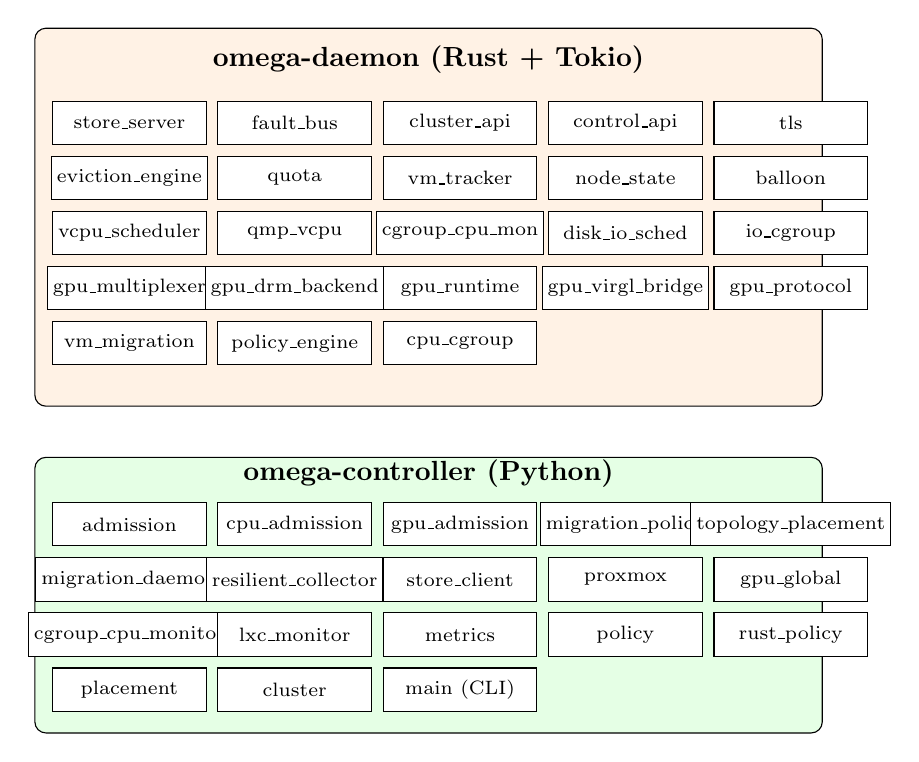
\begin{tikzpicture}[
    daemon/.style={draw, rectangle, rounded corners, fill=orange!10, minimum width=10cm, minimum height=4.8cm, align=center},
    ctrl/.style={draw, rectangle, rounded corners, fill=green!10, minimum width=10cm, minimum height=3.5cm, align=center},
    mod/.style={draw, rectangle, minimum width=1.95cm, minimum height=0.55cm, font=\scriptsize, fill=white, inner sep=2pt}
]
% Démon
\node[daemon] (d) at (0, 3.2) {};
\node[font=\bfseries] at (0, 5.2) {omega-daemon (Rust + Tokio)};

\node[mod] at (-3.8, 4.4) {store\_server};
\node[mod] at (-1.7, 4.4) {fault\_bus};
\node[mod] at ( 0.4, 4.4) {cluster\_api};
\node[mod] at ( 2.5, 4.4) {control\_api};
\node[mod] at ( 4.6, 4.4) {tls};

\node[mod] at (-3.8, 3.7) {eviction\_engine};
\node[mod] at (-1.7, 3.7) {quota};
\node[mod] at ( 0.4, 3.7) {vm\_tracker};
\node[mod] at ( 2.5, 3.7) {node\_state};
\node[mod] at ( 4.6, 3.7) {balloon};

\node[mod] at (-3.8, 3.0) {vcpu\_scheduler};
\node[mod] at (-1.7, 3.0) {qmp\_vcpu};
\node[mod] at ( 0.4, 3.0) {cgroup\_cpu\_mon};
\node[mod] at ( 2.5, 3.0) {disk\_io\_sched};
\node[mod] at ( 4.6, 3.0) {io\_cgroup};

\node[mod] at (-3.8, 2.3) {gpu\_multiplexer};
\node[mod] at (-1.7, 2.3) {gpu\_drm\_backend};
\node[mod] at ( 0.4, 2.3) {gpu\_runtime};
\node[mod] at ( 2.5, 2.3) {gpu\_virgl\_bridge};
\node[mod] at ( 4.6, 2.3) {gpu\_protocol};

\node[mod] at (-3.8, 1.6) {vm\_migration};
\node[mod] at (-1.7, 1.6) {policy\_engine};
\node[mod] at ( 0.4, 1.6) {cpu\_cgroup};

% Contrôleur
\node[ctrl] (c) at (0, -1.6) {};
\node[font=\bfseries] at (0, -0.05) {omega-controller (Python)};

\node[mod] at (-3.8, -0.7) {admission};
\node[mod] at (-1.7, -0.7) {cpu\_admission};
\node[mod] at ( 0.4, -0.7) {gpu\_admission};
\node[mod] at ( 2.5, -0.7) {migration\_policy};
\node[mod] at ( 4.6, -0.7) {topology\_placement};

\node[mod] at (-3.8, -1.4) {migration\_daemon};
\node[mod] at (-1.7, -1.4) {resilient\_collector};
\node[mod] at ( 0.4, -1.4) {store\_client};
\node[mod] at ( 2.5, -1.4) {proxmox};
\node[mod] at ( 4.6, -1.4) {gpu\_global};

\node[mod] at (-3.8, -2.1) {cgroup\_cpu\_monitor};
\node[mod] at (-1.7, -2.1) {lxc\_monitor};
\node[mod] at ( 0.4, -2.1) {metrics};
\node[mod] at ( 2.5, -2.1) {policy};
\node[mod] at ( 4.6, -2.1) {rust\_policy};

\node[mod] at (-3.8, -2.8) {placement};
\node[mod] at (-1.7, -2.8) {cluster};
\node[mod] at ( 0.4, -2.8) {main (CLI)};
\end{tikzpicture}
\caption{Diagramme de composants : démon Rust (haut) et contrôleur Python (bas).}
\label{fig:arch-composants}
\end{figure}

\subsection{Diagramme de déploiement}

La figure~\ref{fig:arch-deploiement} représente le déploiement type sur un cluster Proxmox de quatre nœuds avec Ceph répliqué, conforme à la photographie matérielle de \emph{GRIDZERO}. Les VLANs sont séparés : management (1~Gb/s, RJ45), stockage Ceph (10/25~Gb/s SFP+), public (1~Gb/s, RJ45). Le démon ouvre trois ports : 9100 (inter-nœuds TLS), 9200 (cluster API HTTP), 9300 (control API local HTTP).

\begin{figure}[H]
\centering
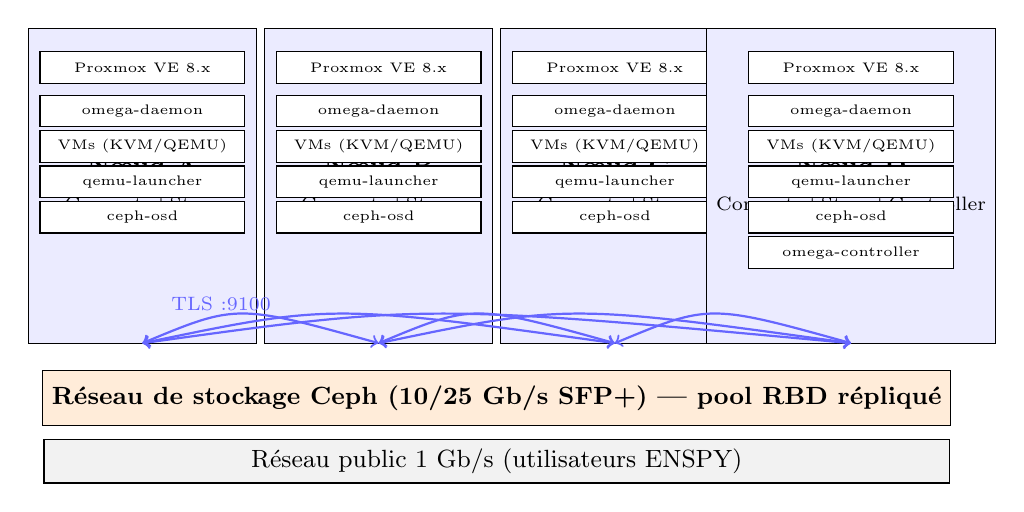
\begin{tikzpicture}[
    host/.style={draw, rectangle, fill=blue!8, minimum width=2.9cm, minimum height=4cm, align=center, font=\small},
    cmp/.style={draw, rectangle, fill=white, minimum width=2.6cm, minimum height=0.4cm, font=\tiny, anchor=center, inner sep=2pt},
    ceph/.style={draw, rectangle, fill=orange!15, minimum width=11.5cm, minimum height=0.7cm, font=\small\bfseries, align=center},
    vlan/.style={draw, dashed, rounded corners, font=\small\itshape}
]
% 4 nœuds
\foreach \x/\name/\role in {-4.5/A/Compute+Store, -1.5/B/Compute+Store, 1.5/C/Compute+Store, 4.5/D/Compute+Store+Controller} {
    \node[host] at (\x, 2.5) {\textbf{Nœud \name}\\[2pt] \scriptsize{\role}};
    \node[cmp] at (\x, 4.0) {Proxmox VE 8.x};
    \node[cmp] at (\x, 3.45) {omega-daemon};
    \node[cmp] at (\x, 3.0) {VMs (KVM/QEMU)};
    \node[cmp] at (\x, 2.55) {qemu-launcher};
    \node[cmp] at (\x, 2.1) {ceph-osd};
}
\node[cmp] at (4.5, 1.65) {omega-controller};

% Ceph
\node[ceph] at (0, -0.2) {Réseau de stockage Ceph (10/25 Gb/s SFP+) --- pool RBD répliqué};

% Liens TLS 9100
\foreach \src/\dst in {-4.5/-1.5, -1.5/1.5, 1.5/4.5, -4.5/4.5, -4.5/1.5, -1.5/4.5} {
    \draw[<->, blue!60, thick] (\src, 0.5) ..controls (\src*0.6+\dst*0.4, 1)..(\dst, 0.5);
}
\node[font=\scriptsize, blue!60] at (-3.5, 1.0) {TLS :9100};

% VLAN public
\node[draw, fill=gray!10, minimum width=11.5cm, minimum height=0.4cm, font=\small, align=center] at (0, -1.0) {Réseau public 1 Gb/s (utilisateurs ENSPY)};
\end{tikzpicture}
\caption{Déploiement type sur cluster Proxmox 4-nœuds avec Ceph.}
\label{fig:arch-deploiement}
\end{figure}

% -----------------------------------------------------------------------------
\section{Conception du paging distant}
\label{sec:conception-paging}

Le paging distant adresse le verrou n\textsuperscript{o}~1 : \emph{la mémoire est cloisonnée par nœud}. Son principe est de détecter, sur un nœud sous pression, les pages froides de ses \acrshort{vm}s, de les envoyer vers la RAM d'un autre nœud, et de les rapatrier de manière transparente lorsqu'elles sont à nouveau accédées.

\subsection{Pipeline d'éviction (Put)}

La figure~\ref{fig:seq-put} décrit la séquence d'éviction d'une page froide. Le déclencheur est la pression mémoire détectée par le \texttt{eviction\_engine} via la lecture périodique de \texttt{/proc/meminfo}.

\begin{figure}[H]
\centering
\begin{tikzpicture}[
    actor/.style={draw, rectangle, minimum width=2cm, minimum height=0.6cm, font=\small\bfseries, fill=blue!10},
    note/.style={font=\scriptsize, align=left},
    msg/.style={->, thick},
    >=Stealth
]
% Acteurs (haut de la séquence)
\node[actor] (engine) at (0, 0)  {EvictionEngine};
\node[actor] (vmtrk)  at (3.2, 0) {VmTracker};
\node[actor] (clock)  at (6.4, 0) {CLOCK};
\node[actor] (peer)   at (9.6, 0) {Store distant};
\node[actor] (kern)   at (12.8, 0) {Kernel};
% Lifelines
\foreach \x in {0, 3.2, 6.4, 9.6, 12.8} {
    \draw[dashed, gray] (\x, -0.4) -- (\x, -6.5);
}
% Messages
\draw[msg] (engine) ++(0,-0.8) -- ++(0,-0.2) node[midway, right, note] {1: lit /proc/meminfo};
\draw[msg] (engine) ++(0,-1.2) -- node[above, note] {2: liste VMs locales} ++(3.2,0);
\draw[msg] (vmtrk)  ++(0,-1.8) -- node[above, note] {3: VMs Running} ++(-3.2,0);
\draw[msg] (engine) ++(0,-2.4) -- node[above, note] {4: sélectionne pages froides} ++(6.4,0);
\draw[msg] (clock)  ++(0,-3.0) -- node[above, note] {5: page\_id froide} ++(-6.4,0);
\draw[msg] (engine) ++(0,-3.8) -- node[above, note] {6: PUT\_PAGE (vm,page,data)} ++(9.6,0);
\draw[msg] (peer)   ++(0,-4.4) -- node[above, note] {7: OK} ++(-9.6,0);
\draw[msg] (engine) ++(0,-5.2) -- node[above, note] {8: madvise(MADV\_DONTNEED)} ++(12.8,0);
\draw[msg] (engine) ++(0,-5.9) -- node[above, note] {9: tracker.mark\_remote(vm,page)} ++(3.2,0);
\end{tikzpicture}
\caption{Diagramme de séquence : éviction d'une page froide.}
\label{fig:seq-put}
\end{figure}

\subsection{Pipeline de récupération (Get)}

La figure~\ref{fig:seq-get} décrit la séquence de récupération d'une page distante, déclenchée par un défaut de page dans la \acrshort{vm}. Cette séquence est sur le \emph{chemin chaud} et conditionne directement la latence perçue par le \emph{guest}.

\begin{figure}[H]
\centering
\begin{tikzpicture}[
    actor/.style={draw, rectangle, minimum width=2cm, minimum height=0.6cm, font=\small\bfseries, fill=blue!10},
    note/.style={font=\scriptsize, align=left},
    msg/.style={->, thick},
    >=Stealth
]
\node[actor] (vm)    at (0, 0)  {VM guest};
\node[actor] (uffd)  at (3, 0)  {userfaultfd};
\node[actor] (bridge) at (6, 0) {uffd-bridge};
\node[actor] (agent) at (9, 0)  {node-a-agent};
\node[actor] (peer)  at (12, 0) {Store distant};
\foreach \x in {0,3,6,9,12} {\draw[dashed, gray] (\x, -0.4) -- (\x, -6.0);}

\draw[msg] (vm)    ++(0,-0.8) -- node[above, note] {1: load (page absente)} ++(3,0);
\draw[msg] (uffd)  ++(0,-1.6) -- node[above, note] {2: uffd\_msg (addr)} ++(3,0);
\draw[msg] (bridge) ++(0,-2.4) -- node[above, note] {3: relais socket uffd.sock} ++(3,0);
\draw[msg] (agent) ++(0,-3.2) -- node[above, note] {4: GET\_PAGE (vm,page\_id)} ++(3,0);
\draw[msg] (peer)  ++(0,-3.9) -- node[above, note] {5: OK + data 4 Kio} ++(-3,0);
\draw[msg] (agent) ++(0,-4.7) -- node[above, note] {6: UFFDIO\_COPY (addr, data)} ++(-6,0);
\draw[msg] (uffd)  ++(0,-5.5) -- node[above, note] {7: reprise du load} ++(-3,0);

\node[note, right] at (12.2, -4.7) {< 5 ms total\\sur GbE};
\end{tikzpicture}
\caption{Diagramme de séquence : récupération d'une page distante.}
\label{fig:seq-get}
\end{figure}

\subsection{Protocole binaire inter-nœuds}

Le canal entre les démons utilise un protocole binaire compact dont l'en-tête fait exactement vingt octets. La figure~\ref{fig:trame} en présente le format précis. Tous les champs multi-octets sont en \emph{big-endian} (convention réseau).

\begin{figure}[H]
\centering
\begin{tikzpicture}[
    fld/.style={draw, rectangle, minimum height=0.7cm, font=\small, align=center}
]
\node[fld, minimum width=2cm]    (m)  at (0,0)    {magic\\ 2 o};
\node[fld, minimum width=1.2cm, right=0pt of m]  (op) {op\\ 1 o};
\node[fld, minimum width=1.2cm, right=0pt of op] (fl) {flag\\ 1 o};
\node[fld, minimum width=2cm,  right=0pt of fl]   (vm) {vm\_id\\ 4 o};
\node[fld, minimum width=2.6cm, right=0pt of vm]  (pg) {page\_id\\ 8 o};
\node[fld, minimum width=2cm,  right=0pt of pg]   (ln) {payload\_len\\ 4 o};
\node[fld, minimum width=4cm,  right=0pt of ln, fill=blue!10]   (pl) {payload\\ jusqu'à 8 192 o};
\draw[<->] (m.south west) ++(0,-0.3) -- node[below, font=\scriptsize] {En-tête fixe 20 octets} ++(8.0, 0);
\end{tikzpicture}
\caption{Format de trame du protocole inter-nœuds (magic \texttt{0x524D}, \og{}RM\fg{}).}
\label{fig:trame}
\end{figure}

Les opcodes définis sont : \texttt{PING}~(\texttt{0x01}), \texttt{PUT\_PAGE}~(\texttt{0x10}), \texttt{GET\_PAGE}~(\texttt{0x11}), \texttt{DELETE\_PAGE}~(\texttt{0x12}), \texttt{BATCH\_PUT\_PAGE}~(\texttt{0x13}), \texttt{STATS\_REQUEST}~(\texttt{0x20}), \texttt{PONG}~(\texttt{0x02}), \texttt{OK}~(\texttt{0x80}), \texttt{NOT\_FOUND}~(\texttt{0x81}), \texttt{ERROR}~(\texttt{0x82}), \texttt{BATCH\_PUT\_OK}~(\texttt{0x83}), \texttt{STATS\_RESPONSE}~(\texttt{0x21}). Le bit \texttt{FLAG\_COMPRESSED} (\texttt{0x01}) signale que le payload est compressé en LZ4 (préfixé par sa taille originale en \emph{u32} big-endian) ; la compression est activée si \texttt{payload.len() \(\ge\) 64} octets et si la version compressée est strictement plus courte. La taille maximale d'un payload simple est de \texttt{MAX\_PAYLOAD = 8192} octets (protection contre les attaques par déni de service) ; pour un \texttt{BATCH\_PUT\_PAGE}, la limite est \texttt{MAX\_BATCH\_PAYLOAD = 262144} octets (64 pages au plus). La constante \texttt{MAGIC = 0x524D} (\og{}RM\fg{} pour \emph{Remote Memory}) identifie le protocole.

\subsection{Algorithme CLOCK avec boucle adaptative}

L'algorithme d'éviction CLOCK, sa boucle de scrutation périodique et sa modulation adaptative par le \texttt{fault\_bus} sont consignés dans l'algorithme~\ref{algo:eviction}.

\begin{algorithm}[H]
\caption{Boucle d'éviction adaptative (\texttt{EvictionEngine})}
\label{algo:eviction}
\KwData{Seuil de pression \(\theta = 75{,}0\%\) ; intervalles \((I_{\text{base}}, I_{\text{accel}}) = (10, 2)\) s ; bus de défauts \(B\) ; limite migrations par cycle \(L = 1\)}
\KwResult{Pages froides évincées ; migrations déclenchées}
$I \gets I_{\text{base}}$\;
\While{le démon est actif}{
   $\text{usage} \gets$ lit \texttt{/proc/meminfo} et calcule $(\text{MemTotal}-\text{MemAvailable})/\text{MemTotal}$\;
   \If{$B$ signale une pression de défauts ($F_{\text{remote}} > \text{seuil}$)}{
       $I \gets I_{\text{accel}}$\;
   } \Else{
       $I \gets I_{\text{base}}$\;
   }
   \If{$\text{usage} \ge \theta$}{
       $\mathcal{V} \gets$ liste des VMs locales en état \emph{Running} (via \texttt{VmTracker})\;
       \ForEach{$v \in \mathcal{V}$}{
           $p \gets$ \texttt{CLOCK.select\_cold\_page}(v) \tcp*{aiguille circulaire, bit accessed}
           \If{$p \ne \bot$}{
               $\text{target} \gets$ choisit un store par \texttt{hash}($v$,$p$) \texttt{\% num\_stores}\;
               envoie \texttt{PUT\_PAGE}(v, p, data) à \emph{target}\;
               appelle \texttt{madvise(MADV\_DONTNEED)} sur la page locale\;
               \texttt{VmTracker.mark\_remote}(v, p)\;
           }
       }
       \If{$\text{usage} \ge \theta + 10\%$ \textbf{et} migrations déclenchées $< L$}{
          consulte \texttt{MigrationPolicy} et déclenche au plus une migration\;
       }
   }
   attend $I$ secondes\;
}
\end{algorithm}

La boucle adaptative est un mécanisme central. Lorsque le \texttt{fault\_bus} (consommateur des événements \texttt{userfaultfd}) indique que le taux de défauts distants \(F_{\text{remote}}\) dépasse un seuil configurable, l'intervalle de scrutation passe de 10\,s à 2\,s : le moteur évince plus agressivement pour anticiper la pression, ce qui réduit le risque d'épuisement complet de la RAM locale et donc la nécessité d'une migration coûteuse.

\subsection{Distribution des pages entre nœuds}

La distribution des pages entre les stores du cluster est \emph{déterministe} : pour une paire $(v, p)$, le store cible est calculé par :
$$\text{target}(v, p) = \text{stores}[\,\mathrm{hash}(v, p) \bmod N\,]$$
où $N$ est le nombre de stores. Cette détermination présente deux avantages : (i) à la récupération, l'agent calcule le même hash et interroge directement le bon store sans annuaire centralisé ; (ii) la répartition est équilibrée statistiquement à mesure que le nombre de pages croît, ce qui évite les hot-spots.

Un facteur de réplication $R \ge 1$ peut être configuré via la variable d'environnement \texttt{OMEGA\_REPLICATION\_FACTOR}. Pour $R=2$, chaque page est envoyée à deux stores distincts (typiquement, target et target+1 modulo $N$). Cela double le coût d'éviction mais permet à la \acrshort{vm} de continuer même si un store tombe.

\subsection{Quota strict : invariant \(\text{local} + \text{remote} \le M_{\max}\)}

Le \texttt{QuotaRegistry} maintient pour chaque \acrshort{vm} une structure \texttt{VmQuota} \{vm\_id, max\_mem\_mib, local\_budget\_mib, remote\_budget\_mib, remote\_used\_mib\} avec l'invariant :
$$\forall v: \quad \mathrm{local\_used}(v) + \mathrm{remote\_used}(v) \le M_{\max}(v) \quad \text{et} \quad \mathrm{remote\_budget}(v) = M_{\max}(v) - \mathrm{local\_budget}(v)$$
L'invariant est vérifié à chaque \texttt{PUT\_PAGE} (algorithme~\ref{algo:quota}). Si l'invariant serait violé, la page est refusée et l'événement est journalisé.

\begin{algorithm}[H]
\caption{Vérification du quota à l'admission d'une page (\texttt{Quota::check\_put})}
\label{algo:quota}
\KwData{VM $v$, taille de page $s$ (4096 octets) ; quota courant $\mathcal{Q}[v]$}
\KwResult{\textsc{Allowed} ou \textsc{Exceeded} ou \textsc{NoQuota}}
\If{$v \notin \mathcal{Q}$}{\Return{\textsc{NoQuota}}\;}
$q \gets \mathcal{Q}[v]$\;
$\text{extra\_mib} \gets s \cdot 1{,}0 / (1024 \cdot 1024)$\;
\If{$q.\text{remote\_used\_mib} + \text{extra\_mib} \le q.\text{remote\_budget\_mib}$}{\Return{\textsc{Allowed}}\;}
\Else{\Return{\textsc{Exceeded}\{$v$, used=$q.\text{remote\_used\_mib}$, budget=$q.\text{remote\_budget\_mib}$\}}\;}
\end{algorithm}

% -----------------------------------------------------------------------------
\section{Conception de l'élasticité}
\label{sec:conception-elasticite}

\subsection{Scheduler vCPU : machine à états et hotplug}

Le scheduler vCPU implémente une machine à états par \acrshort{vm} dont les transitions sont gouvernées par des seuils numériques calibrés. La figure~\ref{fig:vcpu-fsm} décrit la machine et le tableau~\ref{tab:vcpu-seuils} récapitule les seuils.

\begin{figure}[H]
\centering
\begin{tikzpicture}[
    state/.style={draw, rectangle, rounded corners, fill=blue!10, minimum width=2.4cm, minimum height=0.8cm, align=center, font=\small},
    >=Stealth
]
\node[state] (idle)   at (0, 0)   {\textbf{Idle}\\ usage $<$ 35\%};
\node[state] (steady) at (3.5, 0) {\textbf{Steady}\\ 35--80\%};
\node[state] (grow)   at (7, 0)   {\textbf{Growing}\\ $\ge$ 80\%};
\node[state] (throt)  at (10.5, 0){\textbf{Throttled}\\ steal $>$ 10\%};
\node[state] (migr)   at (7, -2.5){\textbf{Migrating}\\ vers autre nœud};

\draw[->] (idle) -- node[above, font=\scriptsize] {usage $\uparrow$} (steady);
\draw[->] (steady) -- node[above, font=\scriptsize] {usage $\ge$ 80\%} (grow);
\draw[->] (grow.south west) ..controls (4, -1)..node[below, font=\scriptsize, sloped] {hotplug OK} (steady.south);
\draw[->] (grow) -- node[above, font=\scriptsize] {steal} (throt);
\draw[->] (throt) -- node[right, font=\scriptsize] {hotplug KO} (migr);
\draw[->] (grow) -- node[right, font=\scriptsize] {saturé} (migr);
\draw[->] (steady.south west) ..controls (1.5, -1)..node[below, font=\scriptsize, sloped] {60s sous 35\%} (idle.south east);
\draw[->] (migr.east) ..controls (10, -2)..node[below, font=\scriptsize] {migration OK} (idle.south west);
\end{tikzpicture}
\caption{Machine à états du scheduler vCPU par VM.}
\label{fig:vcpu-fsm}
\end{figure}

\begin{table}[H]
\centering
\small
\begin{tabular}{llp{6.5cm}}
\toprule
\textbf{Constante} & \textbf{Valeur} & \textbf{Rôle} \\
\midrule
\texttt{VCPU\_PER\_PCPU}          & 3      & Sur-allocation vCPU par cœur physique \\
\texttt{MAX\_VMS\_PER\_SLOT}      & 3      & VMs partageant un même slot \\
\texttt{HOTPLUG\_TRIGGER\_PCT}    & 80,0\% & Déclenche un \emph{hotplug} vCPU \\
\texttt{DOWNSCALE\_TRIGGER\_PCT}  & 35,0\% & Déclenche un retrait vCPU \\
\texttt{DOWNSCALE\_STABLE\_SECS}  & 60     & Durée minimale sous charge faible \\
\texttt{STEAL\_THRESHOLD\_PCT}    & 10,0\% & Steal au-delà $\Rightarrow$ migration prioritaire \\
\texttt{DONOR\_SAFE\_STEAL\_PCT}  & 5,0\%  & Steal max d'une VM donneuse \\
\texttt{DEFAULT\_CPU\_WEIGHT}     & 100    & Poids cgroup nominal \\
\texttt{BOOSTED\_CPU\_WEIGHT}     & 200    & Poids cgroup VM sous pression \\
\texttt{DONOR\_CPU\_WEIGHT}       & 50     & Poids cgroup VM idle \\
\bottomrule
\end{tabular}
\caption{Seuils calibrés du scheduler vCPU.}
\label{tab:vcpu-seuils}
\end{table}

L'algorithme~\ref{algo:vcpu} formalise la boucle de décision principale.

\begin{algorithm}[H]
\caption{Boucle d'ajustement vCPU par VM (\texttt{VcpuScheduler::tick})}
\label{algo:vcpu}
\KwData{VM $v$ avec état $s$ ; $u \gets$ usage CPU cgroup ; $st \gets$ steal time du nœud}
\If{$st > \texttt{STEAL\_THRESHOLD\_PCT}$}{
   marque $v.\text{cpu\_pressure} \gets \textsc{true}$ et notifie \texttt{MigrationPolicy}\;
}
\If{$u \ge \texttt{HOTPLUG\_TRIGGER\_PCT}$ \textbf{et} $s.\text{current} < s.\text{max}$}{
   $slot \gets$ trouver un slot libre (localité même pCPU prioritaire)\;
   \If{$slot \ne \bot$}{
       envoyer \texttt{device\_add cpu} via QMP $\rightarrow s.\text{current} \mathrel{+}= 1$\;
   } \Else{
       déclencher migration prioritaire de $v$\;
   }
}
\If{$u \le \texttt{DOWNSCALE\_TRIGGER\_PCT}$ pendant \texttt{DOWNSCALE\_STABLE\_SECS}}{
   $\text{floor} \gets \max(s.\text{min}, \lceil u / 35{,}0 \rceil)$\;
   \If{$s.\text{current} > \text{floor}$}{
       envoyer \texttt{device\_del cpu} via QMP $\rightarrow s.\text{current} \mathrel{-}= 1$\;
   }
}
\If{une VM borrower demande des cycles \textbf{et} une VM donor existe}{
   ajuster \texttt{cpu.weight} : donor $\gets 50$, borrower $\gets 200$\;
}
\end{algorithm}

\subsection{Scheduler disque : pondération adaptative}

Le scheduler disque suit une logique analogue, mais sans \emph{hotplug} : l'unique levier est le poids cgroup \texttt{io.weight} qui pondère la file d'attente du bloc kernel. Les seuils sont consignés dans le tableau~\ref{tab:disk-seuils} et l'algorithme~\ref{algo:disk} décrit la boucle.

\begin{table}[H]
\centering
\small
\begin{tabular}{llp{6.0cm}}
\toprule
\textbf{Constante} & \textbf{Valeur} & \textbf{Rôle} \\
\midrule
\texttt{DEFAULT\_IO\_WEIGHT}        & 100        & Poids nominal \\
\texttt{BOOSTED\_IO\_WEIGHT}        & 200        & VM active prioritaire \\
\texttt{DONOR\_IO\_WEIGHT}          & 50         & VM idle \\
\texttt{DISK\_PRESSURE\_TRIGGER\_PCT} & 5,0\%    & PSI io.some.avg10 d'activation \\
\texttt{DISK\_BORROWER\_TRIGGER\_BPS} & 8 Mio/s  & Seuil d'activité haute \\
\texttt{DISK\_IDLE\_BPS}            & 512 Kio/s  & Seuil d'inactivité \\
\texttt{DISK\_IDLE\_STABLE\_SECS}   & 60         & Durée avant rétrogradation \\
\bottomrule
\end{tabular}
\caption{Seuils du scheduler I/O disque.}
\label{tab:disk-seuils}
\end{table}

\begin{algorithm}[H]
\caption{Boucle d'arbitrage I/O (\texttt{DiskIoScheduler::tick})}
\label{algo:disk}
\KwData{Pression nœud $\pi \gets$ PSI io.some.avg10}
\ForEach{VM $v$ locale}{
   $r, w \gets$ lit \texttt{io.stat} cgroup et calcule $rb, wb$ en bytes/s\;
   $tot \gets rb + wb$\;
   \If{$\pi \ge \texttt{DISK\_PRESSURE\_TRIGGER\_PCT}$ \textbf{et} $tot \ge \texttt{DISK\_BORROWER\_TRIGGER\_BPS}$}{
       écrire \texttt{BOOSTED\_IO\_WEIGHT} dans \texttt{io.weight} de $v$\;
   }
   \If{$tot \le \texttt{DISK\_IDLE\_BPS}$ pendant \texttt{DISK\_IDLE\_STABLE\_SECS}}{
       écrire \texttt{DONOR\_IO\_WEIGHT} dans \texttt{io.weight} de $v$\;
   }
}
\end{algorithm}

\subsection{Multiplexeur GPU : file unique, leader-election, budget VRAM}

Le multiplexeur GPU adresse le verrou n\textsuperscript{o}~3 (\acrshort{gpu} en passthrough exclusif). Son principe est de remplacer le passthrough par un \emph{accès médié} : les \acrshort{vm}s n'attaquent pas le \acrshort{gpu} directement, mais envoient des requêtes (\emph{Submit}, \emph{Alloc}, \emph{Free}) sur une socket Unix \texttt{/run/omega/gpu.sock} ; le démon les arbitre puis appelle le pilote DRM réel via \texttt{/dev/dri/renderD128}.

La sérialisation par une \emph{file de priorité unique globale} (\texttt{BinaryHeap} triée par couple (priorité~\textsc{desc}, timestamp~\textsc{asc})) est imposée par l'architecture matérielle : un \acrshort{gpu} n'est pas \emph{thread-safe} pour des soumissions concurrentes. Quatre niveaux de priorité sont définis : \textsc{Low}~(0), \textsc{Normal}~(1), \textsc{High}~(2), \textsc{RealTime}~(3). La leader-election par \texttt{flock} sur \texttt{/run/omega-gpu-scheduler-<pci>.lock} garantit qu'un seul démon par nœud orchestre un \acrshort{gpu} donné.

Le format binaire \texttt{GpuHeader} sur la socket comporte : magic \texttt{0x4F4D4750} (\og{}OMGP\fg{}), version, \texttt{vm\_id}, numéro de séquence, \texttt{payload\_len}, priorité (22 octets en-tête + payload). L'algorithme~\ref{algo:gpu} résume la boucle d'arbitrage.

\begin{algorithm}[H]
\caption{Multiplexeur GPU --- boucle d'arbitrage}
\label{algo:gpu}
\KwData{Heap $H$ ; budgets \texttt{vram\_budget}, \texttt{vram\_used} par VM ; backend DRM}
\While{le démon est actif}{
   \If{$H$ non vide}{
       $(msg, reply) \gets H.\text{pop}()$\;
       \Switch{$msg.\text{type}$}{
          \Case{\textsc{AllocRequest}($size$)}{
              \eIf{$\text{vram\_used}[v] + size > \text{vram\_budget}[v]$}{
                 répondre \textsc{OutOfVram}\;
              }{
                 $h \gets$ DRM\_GEM\_ALLOC($size$)\;
                 $\text{vram\_used}[v] \mathrel{+}= size$\;
                 répondre OK + $h$\;
              }
          }
          \Case{\textsc{FreeRequest}($h$)}{
              DRM\_GEM\_FREE($h$)\;
              $\text{vram\_used}[v] \mathrel{-}= \text{size}(h)$\;
          }
          \Case{\textsc{Submit}($cmd$)}{
              soumettre la \emph{command stream} via DRM ; répondre fence\;
          }
       }
   } \Else{
       attendre nouveau message sur la socket\;
   }
}
\end{algorithm}

\subsection{Balloon : thin-provisioning piloté par taux de défauts}

Le \texttt{balloon} virtio~\cite{qemu_balloon,waldspurger_2002} permet d'ajuster dynamiquement la mémoire \emph{visible} par la \acrshort{vm}. Notre conception en fait un mécanisme de \emph{thin-provisioning} : une \acrshort{vm} démarre avec \texttt{balloon\_initial\_mib} (défaut 512~Mio) et croît progressivement jusqu'à \texttt{region\_mib} (plafond fixé à la création) en fonction du \emph{taux de défauts de page par seconde}. La règle est simple : si \texttt{fault\_rate $\ge$ grow\_faults\_per\_sec}, on commande \texttt{qm balloon vmid (mib+step)} ; si \texttt{fault\_rate $\le$ shrink\_faults\_per\_sec}, on récupère. L'intérêt est qu'aucune RAM n'est réservée sur les stores tant que les pages ne sont pas effectivement accédées.

% -----------------------------------------------------------------------------
\section{Conception de la migration automatique}
\label{sec:conception-migration}

\subsection{Diagramme d'activité de la décision live/cold}

La figure~\ref{fig:decision-migration} décrit l'arbre de décision live vs cold appliqué par \texttt{MigrationPolicy} au sein du contrôleur.

\begin{figure}[H]
\centering
\begin{tikzpicture}[
    decision/.style={draw, diamond, aspect=2, fill=yellow!15, font=\small, align=center, inner sep=1pt},
    action/.style={draw, rectangle, rounded corners, fill=green!15, font=\small, align=center, minimum height=0.7cm},
    start/.style={draw, circle, fill=black, minimum size=0.3cm, inner sep=0pt},
    >=Stealth
]
\node[start] (s) at (0,3.5) {};
\node[decision] (d1) at (0,2.5) {RAM $>$ 95\,\% ?};
\node[action]   (a1) at (4.5,2.5) {COLD forcée};
\node[decision] (d2) at (0,1.0) {RAM $>$ 85\,\% ?};
\node[decision] (d3) at (4.5,1.0) {VM idle $>$ 60\,s ?};
\node[action]   (a2) at (4.5,-0.3) {COLD};
\node[action]   (a3) at (8.5,1.0) {LIVE};
\node[decision] (d4) at (0,-0.5) {throttle $>$ 30\,\% ?};
\node[action]   (a4) at (4.5,-1.6) {LIVE};
\node[action]   (a5) at (0,-1.8) {Aucune migration};

\draw[->] (s) -- (d1);
\draw[->] (d1) -- node[above, font=\scriptsize] {oui} (a1);
\draw[->] (d1) -- node[right, font=\scriptsize] {non} (d2);
\draw[->] (d2) -- node[above, font=\scriptsize] {oui} (d3);
\draw[->] (d2) -- node[right, font=\scriptsize] {non} (d4);
\draw[->] (d3) -- node[right, font=\scriptsize] {oui} (a2);
\draw[->] (d3) -- node[above, font=\scriptsize] {non} (a3);
\draw[->] (d4) -- node[above, font=\scriptsize] {oui} (a4);
\draw[->] (d4) -- node[right, font=\scriptsize] {non} (a5);
\end{tikzpicture}
\caption{Décision de migration : live vs cold vs abstention.}
\label{fig:decision-migration}
\end{figure}

Les seuils calibrés exacts de \texttt{MigrationPolicy} sont consignés dans le tableau~\ref{tab:migration-seuils}.

\begin{table}[H]
\centering
\small
\begin{tabular}{llp{7cm}}
\toprule
\textbf{Seuil} & \textbf{Valeur} & \textbf{Effet} \\
\midrule
\texttt{ram\_high\_pct}         & 85\%        & Migrer LIVE \\
\texttt{ram\_critical\_pct}     & 95\%        & Forcer COLD (live ne convergerait pas) \\
\texttt{vcpu\_throttle\_trigger} & 30\%       & Migrer LIVE (libérer cycles) \\
\texttt{vcpu\_saturation\_pct}  & 90\%        & Migrer LIVE \\
\texttt{remote\_paging\_pct}    & 60\%        & Migrer LIVE (trop de pages distantes) \\
\texttt{disk\_high\_pct}        & 10\%        & PSI io.avg10 déclenche évaluation \\
\texttt{idle\_cpu\_pct}         & 5,0\%       & VM idle si CPU $<$ ce seuil \\
\texttt{idle\_duration\_secs}   & 60          & Durée avant cold viable \\
\texttt{target\_max\_ram\_pct}  & 80\%        & Nœud cible peut monter jusqu'à ce niveau \\
\texttt{target\_max\_vcpu\_pct} & 80\%        & Idem pour vCPU \\
\bottomrule
\end{tabular}
\caption{Seuils de \texttt{MigrationPolicy}.}
\label{tab:migration-seuils}
\end{table}

\subsection{Score de placement multi-critères}

Le choix du nœud cible se fait par maximisation d'un score $S(n)$ multi-critères pondéré :

\begin{equation}
\boxed{\;
S(n) \;=\; 0{,}50 \cdot S_{\text{RAM}}(n) \;+\; 0{,}25 \cdot S_{\text{topo}}(n) \;+\; 0{,}15 \cdot S_{\text{CPU}}(n) \;+\; 0{,}10 \cdot S_{\text{mig}}(n)
\;}
\label{eq:score}
\end{equation}

Les composantes sont définies comme suit :

\begin{itemize}[leftmargin=*]
    \item $S_{\text{RAM}}(n) = \min\!\left(1, \dfrac{\text{free}(n) - \text{required}}{\text{max\_free\_cluster}}\right)$ : récompense la marge mémoire disponible \emph{au-delà} du strict nécessaire ;
    \item $S_{\text{topo}}(n)$ : prend la valeur $1{,}00$ pour \emph{même rack}, $0{,}65$ pour \emph{même zone}, $0{,}20$ pour \emph{cross-zone}, pénalisé linéairement si la latence inter-nœuds dépasse 50~ms ;
    \item $S_{\text{CPU}}(n) = 1 - \text{cpu\_usage}(n)$ : favorise les nœuds peu chargés ;
    \item $S_{\text{mig}}(n) = \dfrac{1}{1 + \text{active\_migrations}(n)}$ : pénalise les nœuds déjà engagés dans une migration.
\end{itemize}

Cette pondération a été itérée empiriquement : la prédominance de la RAM (50~\%) reflète le fait qu'une migration consommatrice se justifie d'abord par un risque de saturation mémoire, le critère topologique (25~\%) intervient pour limiter la latence sur les charges sensibles, le critère CPU (15~\%) sert d'arbitrage secondaire, et la pénalisation des migrations actives (10~\%) évite les phénomènes de \emph{cascade}.

\subsection{Cleanup post-migration}

Toute migration réussie déclenche un cleanup sur le nœud source pour libérer les ressources désormais inutiles. L'algorithme~\ref{algo:cleanup} résume les actions :

\begin{algorithm}[H]
\caption{Cleanup après migration réussie}
\label{algo:cleanup}
\KwData{VM $v$ migrée du nœud source vers la cible}
supprimer toutes les pages $(v, *)$ du store local\;
notifier les stores distants : \texttt{DELETE\_PAGE}($v$, $*$) (pages possédées par $v$)\;
libérer les slots vCPU occupés par $v$ dans le scheduler\;
retirer le quota mémoire de $v$ du \texttt{QuotaRegistry}\;
libérer le budget VRAM de $v$ du multiplexeur GPU\;
supprimer $v$ du \texttt{VmTracker} local\;
journaliser l'événement \texttt{migration\_completed} avec durée et raison\;
\end{algorithm}

\subsection{Veto absolu GPU}

Le score $S(n)$ est complété par un \emph{veto absolu} : si la \acrshort{vm} à migrer requiert un \acrshort{gpu} (configuré via \texttt{hostpci0}) et que le nœud candidat ne dispose d'aucun \acrshort{gpu} avec suffisamment de \acrshort{vram} libre, alors $S(n)$ est forcé à $-\infty$ et le nœud est exclu de la sélection. Cette règle est non-négociable et précède l'évaluation du score.

% -----------------------------------------------------------------------------
\section{Conception de l'admission et de la collecte résiliente}
\label{sec:conception-admission}

\subsection{Admission RAM, vCPU, GPU}

L'admission d'une nouvelle \acrshort{vm} se fait au niveau cluster par le contrôleur (\texttt{admission.py}, \texttt{cpu\_admission.py}, \texttt{gpu\_admission.py}). L'algorithme~\ref{algo:admission} synthétise la séquence :

\begin{algorithm}[H]
\caption{Admission d'une nouvelle VM (vue cluster-wide)}
\label{algo:admission}
\KwData{Spec VM : $M_{\max}$, $\text{vcpu}_{\min}$, $\text{vcpu}_{\max}$, $\text{vram}$ ; cluster $\mathcal{C}$ ; safety\_margin = 10\%}
\KwResult{(nœud cible, local\_budget, remote\_budget) ou REFUS}
$\text{cluster\_free\_ram} \gets \sum_{n \in \mathcal{C}} \text{free\_ram}(n)$\;
\If{$\text{cluster\_free\_ram} < M_{\max}$}{\Return{\textsc{Refus} (RAM)}\;}
$\text{cluster\_free\_vcpu} \gets$ slots libres totaux (3 vCPU × 3 VMs / pCPU)\;
\If{$\text{vcpu}_{\min} > \text{cluster\_free\_vcpu}$}{\Return{\textsc{Refus} (vCPU)}\;}
\If{$\text{vram} > 0$ \textbf{et} aucun nœud n'a $\text{vram\_free} \ge \text{vram}$}{\Return{\textsc{Refus} (VRAM)}\;}
$\mathcal{N}_{\text{ok}} \gets$ nœuds satisfaisant les contraintes vCPU et VRAM\;
$n^* \gets \arg\max_{n \in \mathcal{N}_{\text{ok}}} S(n)$ (cf. eq.~\ref{eq:score})\;
$\text{local\_budget} \gets \min\!\bigl(\text{free\_ram}(n^*) \cdot (1 - 0{,}10),\, M_{\max}\bigr)$\;
$\text{remote\_budget} \gets M_{\max} - \text{local\_budget}$\;
envoyer la config quota au démon de $n^*$ via \texttt{POST /control/admit}\;
\Return{$(n^*, \text{local\_budget}, \text{remote\_budget})$}\;
\end{algorithm}

\subsection{Collecte résiliente avec circuit-breaker}

Le contrôleur interroge les démons via HTTP avec une protection par \emph{circuit-breaker}~\cite{nygard_release} à trois états (\textsc{Closed}, \textsc{Open}, \textsc{HalfOpen}) et un cache de fraîcheur 120~secondes. La figure~\ref{fig:circuit} décrit la machine à états du \emph{circuit-breaker}.

\begin{figure}[H]
\centering
\begin{tikzpicture}[
    state/.style={draw, rectangle, rounded corners, fill=blue!10, minimum width=2.6cm, minimum height=0.8cm, align=center, font=\small},
    >=Stealth
]
\node[state] (closed) at (0, 0)   {\textbf{Closed}\\ requêtes passent};
\node[state] (open)   at (5, 0)   {\textbf{Open}\\ requêtes bloquées};
\node[state] (half)   at (10, 0)  {\textbf{HalfOpen}\\ sonde de test};
\draw[->] (closed) -- node[above, font=\scriptsize] {3 échecs consécutifs} (open);
\draw[->] (open)   -- node[above, font=\scriptsize] {après 30 s} (half);
\draw[->] (half)   ..controls (8,-1.8) and (2,-1.8).. node[below, font=\scriptsize, sloped] {sonde OK} (closed);
\draw[->] (half)   ..controls (7.5,1.4)..  node[above, font=\scriptsize] {sonde KO} (open);
\end{tikzpicture}
\caption{Machine à états du \emph{circuit-breaker} de \texttt{ResilientCollector}.}
\label{fig:circuit}
\end{figure}

La politique de retry combine backoff exponentiel (0,5\,s, 1\,s, 2\,s, plafonné à 8\,s) et jitter $\pm$10\,\% pour éviter le \emph{thundering herd}. Si le \emph{circuit} est ouvert, le collecteur retourne le dernier état connu, marqué \texttt{stale=True}. Cette stratégie maximise l'utilité décisionnelle : il est généralement meilleur de raisonner sur des données vieilles de quelques dizaines de secondes que de bloquer le contrôleur sur un \emph{panic}.

% -----------------------------------------------------------------------------
\section{Conception du canal de transport et de la sécurité}
\label{sec:conception-tls}

\subsection{Séparation des plans réseau}

Le système ouvre trois ports distincts, chacun avec un usage et un modèle de menace propres :

\begin{itemize}[leftmargin=*]
    \item \textbf{Port 9100 (TCP + TLS)} : canal inter-nœuds pour le protocole binaire de pages. Chiffrement TLS~1.3 obligatoire, vérification d'identité par empreinte TOFU.
    \item \textbf{Port 9200 (HTTP plain)} : API cluster pour le contrôleur. Plain HTTP toléré car restreint au VLAN management (firewall hôte) ; à terme, migration possible vers HTTPS+mTLS.
    \item \textbf{Port 9300 (HTTP plain, local only)} : canal de contrôle local pour les opérations administratives (éviction, quotas, métriques Prometheus). \emph{Bind} sur \texttt{127.0.0.1} uniquement.
\end{itemize}

\subsection{Empreinte TOFU et premier déploiement}

À la première connexion entre deux nœuds, l'empreinte SHA-256 du certificat du pair est enregistrée dans un fichier local \texttt{/var/lib/omega/tofu/<peer\_id>.fp}. Aux connexions suivantes, l'empreinte présentée est comparée à l'empreinte stockée ; toute divergence est traitée comme une attaque \emph{man-in-the-middle} et la connexion est rejetée. Ce modèle suppose que la première connexion ait lieu dans un environnement de confiance, ce qui est le cas du déploiement initial du cluster GRIDZERO sur un VLAN management isolé.

% -----------------------------------------------------------------------------
\section{Synthèse de la conception}
\label{sec:synthese-conception}

Le tableau~\ref{tab:synth-conception} synthétise les principaux modules conçus, leurs leviers et leurs interfaces externes. Il sert de pivot avec le chapitre~\ref{chap:implementation} qui détaille les implémentations correspondantes.

\begin{table}[H]
\centering
\small
\begin{tabular}{p{3cm}p{3.8cm}p{3.5cm}p{3.2cm}}
\toprule
\textbf{Module} & \textbf{Levier principal} & \textbf{Interfaces ext.} & \textbf{Invariant} \\
\midrule
EvictionEngine    & CLOCK + AdaptiveInterval         & \texttt{/proc/meminfo}, fault\_bus & Seuil 75\% \\
Quota             & Vérif à chaque PUT               & PUT\_PAGE                          & $\text{local}+\text{rem} \le M_{\max}$ \\
StoreServer       & DashMap shardé + TLS             & TCP :9100                          & Taille payload 4096 \\
VcpuScheduler     & QMP hotplug + cgroup weight      & QMP, cgroup, /proc/stat            & vCPU $\in [\min,\max]$ \\
DiskIoScheduler   & \texttt{io.weight} adaptatif     & cgroup, PSI io                     & Poids $\in [1,10000]$ \\
GpuMultiplexer    & File priorité + flock leader     & Unix sock, /dev/dri/renderD*       & 1 leader / GPU \\
VmMigration       & \texttt{qm migrate} + cleanup    & qm, Ceph                           & Cleanup atomique \\
TopologyPlacement & Score multi-critères (eq.~\ref{eq:score}) & \texttt{/control/status}    & $\sum w_i = 1$ \\
MigrationPolicy   & Seuils 85/95/60s                 & status nœuds + score              & 1 décision / cycle \\
ResilientCollector & Circuit-breaker 3-états         & HTTP :9200                         & TTL cache 120\,s \\
\bottomrule
\end{tabular}
\caption{Synthèse des modules conçus.}
\label{tab:synth-conception}
\end{table}


La conception détaillée a été présentée verrou par verrou. Le paging distant repose sur l'algorithme CLOCK alimenté par une boucle adaptative qui réagit au taux de défauts réel, sur un protocole binaire de 20~octets sécurisé par TLS+TOFU, et sur un invariant strict de quota vérifié à chaque opération. L'élasticité combine une machine à états vCPU avec hotplug QMP, un scheduler I/O pondéré par PSI, et un multiplexeur GPU avec leader-election par \texttt{flock}. La migration automatique s'appuie sur un score multi-critères pondéré et un veto GPU absolu. L'admission cluster-wide vérifie la disponibilité RAM/vCPU/VRAM avant de placer une nouvelle \acrshort{vm}. Le chapitre suivant entre dans l'implémentation effective et présente les résultats expérimentaux obtenus.
